\lab{Python}{NumPy Arrays}{NumPy Arrays}
\objective{Create and manipulate powerful NumPy $n$-dimensional arrays.}
\label{lab:NumPyArrays}

\section*{Why Arrays?}
Let's begin with a simple demonstration of why arrays are important for numerical computation.
We know Python already has a reasonably efficient list object, so why use arrays?
In this demonstration, we will square a matrix that is represented as a two dimensional list (i.e. a list of lists).

The following is a function that will accept two matrices (each a two dimensional list), $A$ and $B$ and return $AB$ following the usual rules of matrix multiplication.
\lstinputlisting[style=fromfile]{arr_mult.py}
We can initialize a $k \times k$ ``array" of integers like this:
\begin{lstlisting}
>>> k = 10
>>> A = [range(i, i+k) for i in range(0, k**2, k)]
\end{lstlisting}

\begin{problem}
Time how long NumPy and the \li{arr_mult.py} function listed above takes to square matrices for \li{k = 100, 200, 300} and report the computed times. Briefly comment on the time needed to square a two dimensional list vs. a two dimensional NumPy array.

In IPython you can time how long it takes for a line of code to execute by prefacing it with \li{\%timeit}. The following instruction may be useful in completing this problem. 

Import timeit and NumPy. Create a NumPy array, \li{A}, and square it.
Note that \li{A*A} does \emph{not} square the array using matrix multiplication, but rather multiplies \li{A} with itself element by element.
To get matrix multiplication for NumPy arrays you must use \li{np.dot} or the \li{dot()} method of an array like this:
\begin{lstlisting}
import numpy as np
k=100
A = np.array([range(i, i+k) for i in range(0, k**2, k)])
np.dot(A, A)
\end{lstlisting}
It may be beneficial to write a timer function similar to the following. 
\begin{lstlisting}
import timeit
def timefunction(f, *args, **kwargs):
	pfunc = lambda: f(*args, **kwargs)
	print min(timeit.repeat(pfunc, number = 1, repeat = 3))
\end{lstlisting}
\end{problem}

% Below is a comparison of runtimes needed to square a matrix
% \begin{center}
% \begin{tabular}{|c|l|l|}
% \hline
%  Data Structure & Size & Time (s) \\ \hline
%  Python List & $1\times1$ & 0.0000181198 \\ \cline{2-3}
%       & $10\times10$ & 0.0002758503 \\ \cline{2-3}
%       & $100\times100$ & 0.1336028576 \\ \cline{2-3}
%       & $1000\times1000$ & 200.4009799957 \\ \hline \hline
%  NumPy Array & $1\times1$ & 0.0000298023 \\ \cline{2-3}
%       & $10\times10$ & 0.0000109673 \\ \cline{2-3}
%       & $100\times100$ & 0.0009210110 \\ \cline{2-3}
%       & $1000\times1000$ & 2.1682999134 \\ \hline
% \end{tabular}
%
% \end{center}



The reason for the drastic speed difference is that Python, as a high level interpreted language, tends to be slower than lower level compiled languages.
The algorithms implemented in NumPy are heavily optimized and are usually implemented in C or Fortran.
Instead of operating purely in Python they use Python to run code that is written and optimized in other languages.
NumPy interfaces with some of the best packages available for doing computational linear algebra and can be used to write relatively fast programs.

\section*{NumPy}
NumPy is one of the fundamental packages for scientific computing with Python.
At its heart lies an efficient \li{ndarray} ($n$-dimensional array) object for fast computations.
These arrays form the foundation of all computations done in NumPy and SciPy (a higher-level scientific computing library built on top of NumPy).
NumPy is typically imported like this:
\begin{lstlisting}
>>> import numpy as np
\end{lstlisting}

\section*{Creating Arrays}
The most elementary way to create an array is to define it explicitly using \li{np.array()}.
\begin{lstlisting}
>>> a = np.array([1, 3, 5, 7, 11])
>>> a
array([ 1,  3,  5,  7, 11])
\end{lstlisting}
NumPy provides a variety of ways to easily create different kinds of arrays.
\li{np.arange()} creates a ranged array much the same way that Python's \li{range} statement creates a list.
\begin{lstlisting}
>>> b = np.arange(10)
>>> b
array([0, 1, 2, 3, 4, 5, 6, 7, 8, 9])
\end{lstlisting}
Its optional arguments work the same as the optional arguments do for the \li{range} function that is built into Python.
We can also create arrays that consist entirely of ones or zeros using \li{np.ones()} and \li{np.zeros()} respectively.
\begin{lstlisting}
>>> c = np.ones(5)
>>> c
array([ 1.,  1.,  1.,  1.,  1.])
>>> d = np.zeros(5)
>>> d
array([ 0.,  0.,  0.,  0.,  0.])
\end{lstlisting}
We can even create an array that has evenly spaced numbers over a desired interval.
The first and second arguments define the endpoints of this closed interval.
\begin{lstlisting}
>>> e = np.linspace(0, 32, 4) # 4 values ranging evenly from 0 to 32
>>> e
array([  0.        ,  10.66666667,  21.33333333,  32.        ])
\end{lstlisting}
We can even create arrays using random values chosen from a variety of probability distributions.
These functions are stored in a submodule of NumPy called \li{np.random}.
\begin{lstlisting}
>>> f = np.random.rand(5) #uniformly distributed values
>>> f
array([ 0.21845499,  0.73352537,  0.28064456,  0.66878454,  0.44138609])
>>> f = np.random.randint(0, 5, 6) # 6 randomly generated integers uniformly distributed in [0, 5)
>>> f
array([ 3,  1,  0,  3,  4,  1])
>>> f = np.random.randn(5) #normally distributed values
array([-1.30752235, -0.60518647,  2.08529266, -0.43919065,  0.92830676])
\end{lstlisting}
We can even allocate an array without initializing its values to any value.
This is most useful when the initial values of an array do not matter (like when you are constructing an array filled with specific values or when you are going to overwrite it).
\begin{lstlisting}
>>> g = np.empty(5)
>>> g
array([  0.00000000e+000,   1.30586451e-316,   1.17126324e-316,
         0.00000000e+000,   2.37151510e-322])
\end{lstlisting}
We can also create an array with the same shape and type as another given array.
\begin{lstlisting}
>>> h = np.random.rand(3,5)
>>> h
array([[ 0.90193121,  0.54952824,  0.71892463],
       [ 0.44109638,  0.9431592 ,  0.09779614]])
>>> j = np.empty_like(h)
>>> j
array([[  3.18299369e-313,   4.95065560e+173,  -1.00498695e+047],
       [ -2.88958188e-089,   3.18299369e-313,   7.92118726e-314]])
\end{lstlisting}
Note that you can also dictate that your new array be filled entirely with ones or zeros by using the \li{empty_like} or \li{zeros_like} respectively. 


\section*{Array Objects}
Unlike Python containers, all of the elements of an array must have the same datatype.
These datatypes are machine-native data types that avoid the overhead of Python objects (an \li{int} in NumPy is not the same as an \li{int} in Python).
The benefit of using these machine-native types is a a tremendous speedup of numerical operations.
The datatypes supported by NumPy are shown in Table \ref{numpytypes}
\begin{table}
\begin{tabular}{l|l}
Data type & Description \\
\hline
\li{bool} & Boolean \\
\li{int8} & 8-bit integer \\
\li{int16} & 16-bit integer \\
\li{int32} & 32-bit integer \\
\li{int64} & 64-bit integer \\
\li{int} & Platform integer (depends on platform) \\
\li{uint8} & Unsigned 8-bit integer \\
\li{uint16} & Unsigned 16-bit integer \\
\li{uint32} & Unsigned 32-bit integer \\
\li{uint64} & Unsigned 64-bit integer \\
\li{float16} & Half precision float \\
\li{float32} & Single precision float \\
\li{float64} & Double precision float (also \li{float}) \\
\li{complex64} & Complex number represented by two single precision floats \\
\li{complex128} & Complex number represented by two double precision floats (also \li{complex})
\end{tabular}
\caption{Native numerical data types available in NumPy.}
\label{numpytypes}
\end{table}
Like any other object in Python, \li{ndarray} objects have methods and properties associated with them.
We can derive information from arrays by looking at their different attributes.
The data type of the array can be inferred from the \li{dtype} property.
Many of the array constructors accept an optional \li{dtype} keyword that lets you specify the type of the array to be created.
\begin{lstlisting}
>>> a.dtype
dtype('float64')
>>> a = np.array(range(5), dtype=np.uint8)
>>> a.dtype
dtype('uint8')
\end{lstlisting}
We can check the number of dimensions an array looking at the value of the \li{ndim} property.
\begin{lstlisting}
>>> a.ndim
1
\end{lstlisting}
We can see the sizes of each dimension by looking at the \li{shape} property.
This will return a Python tuple of the size of each dimension.
\begin{lstlisting}
>>> a.shape
(5,)
>>> len(a) #simply returns the size of the first dimension
5
\end{lstlisting}
To know the total number of elements in the array, we can use the \li{size} property
\begin{lstlisting}
>>> a.size
5
\end{lstlisting}
For a single dimensional array, these properties are uninteresting.
These array properties are the most efficient way to understand the size and shape of an array.

Let's look at higher dimensional arrays.
One, two, and three dimensional arrays are easy to visualize.
Higher dimensional NumPy arrays can be thought of as arrays within arrays.
A three dimensional array can just be thought of as an array of arrays of arrays.
The 3D index, \li{A[3, 5, 1]}, essentially means \emph{take the second element of the sixth subarray of the fourth subarray of A}.
Each dimension is called an \emph{axis} in NumPy (ie. a 3D array has 3 axes).  Many of NumPy's functions can be restricted to an axis.
\begin{comment}
Most of the array constructors we have looked so far support creating arrays with an arbitrary number of dimensions.
We can create an identity matrix easily with \li{np.eye}, \li{np.identity}, or \li{np.diag}.
\li{np.eye} is the most versatile and allows for non-square outputs, in which case it puts ones on the diagonal and zeros everywhere else.
\li{np.diag} is an interesting function.  If given an existing array, it will extract the diagonal elements.
However, if given anything else, it will construct a diagonal array and return it.
\begin{lstlisting}
>>> h = np.eye(5)
>>> h
array([[ 1.,  0.,  0.,  0.,  0.],
       [ 0.,  1.,  0.,  0.,  0.],
       [ 0.,  0.,  1.,  0.,  0.],
       [ 0.,  0.,  0.,  1.,  0.],
       [ 0.,  0.,  0.,  0.,  1.]])
>>> np.eye(3, 5)
array([[ 1.,  0.,  0.,  0.,  0.],
       [ 0.,  1.,  0.,  0.,  0.],
       [ 0.,  0.,  1.,  0.,  0.]])
>>> np.identity(3)
array([[ 1.,  0.,  0.],
       [ 0.,  1.,  0.],
       [ 0.,  0.,  1.]])
>>> np.diag(h)
array([ 1.,  1.,  1.,  1.,  1.])
>>> i = np.diag(np.arange(5))
>>> i
array([[0, 0, 0, 0, 0],
       [0, 1, 0, 0, 0],
       [0, 0, 2, 0, 0],
       [0, 0, 0, 3, 0],
       [0, 0, 0, 0, 4]])
\end{lstlisting}
Another powerful function is \li{np.tile()}.
This allows us to tile arrays across one or more dimensions.
\begin{lstlisting}
>>> j = np.array([1, 9, 5, 2])
>>> np.tile(j, 3)
array([1, 9, 5, 2, 1, 9, 5, 2, 1, 9, 5, 2])
>>> k = np.tile(j, (3, 3, 2))
>>> k
array([[[1, 9, 5, 2, 1, 9, 5, 2],
        [1, 9, 5, 2, 1, 9, 5, 2],
        [1, 9, 5, 2, 1, 9, 5, 2]],

       [[1, 9, 5, 2, 1, 9, 5, 2],
        [1, 9, 5, 2, 1, 9, 5, 2],
        [1, 9, 5, 2, 1, 9, 5, 2]],

       [[1, 9, 5, 2, 1, 9, 5, 2],
        [1, 9, 5, 2, 1, 9, 5, 2],
        [1, 9, 5, 2, 1, 9, 5, 2]]])
\end{lstlisting}

\end{comment}

It is also often useful to create arrays that represent a two-dimensional grid of coordinates.
This is done using the \li{meshgrid()} function, for example:
\begin{lstlisting}
>>> x = np.arange(4)
>>> y = np.arange(4, 8)
>>> X, Y = np.meshgrid(x, y)
>>> X
array([[0, 1, 2, 3],
       [0, 1, 2, 3],
       [0, 1, 2, 3],
       [0, 1, 2, 3]])
>>> Y
array([[4, 4, 4, 4],
       [5, 5, 5, 5],
       [6, 6, 6, 6],
       [7, 7, 7, 7]])
\end{lstlisting}
As you can see, \li{X} is an array representing the $x$ coordinates for a grid of points and \li{Y} is an array representing the $y$ coordinates of that same grid of points.
\begin{comment}
When creating large grids of points this can use large amounts of RAM, so the meshgrid function includes the \li{copy} argument which, when set to false, returns arrays that are views of the original arrays instead of copies (views and copies are discussed later in this lab).
For example, instead of running \li{np.meshgrid(x, y)} you could run \li{np.meshgrid(x, y, copy=False)}.
This can be much faster, but should probably only be used if you do not intend to make any additional changes to the coordinates grid independent of the values stored in the original arrays.

Every NumPy array has five flags that give important information about the array.
We can check if an array is read-only by looking at its flags, or we can check how the array's contents are laid out in memory.
Only the \texttt{WRITEABLE} and \texttt{ALIGNED} flags can be modified.  The other flags are read-only.
The \texttt{OWNDATA} flag lets us know if the array is a view or not.
We will explain array views later in this lab.
\begin{lstlisting}
>>> i.flags
  C_CONTIGUOUS : True
  F_CONTIGUOUS : False
  OWNDATA : True
  WRITEABLE : True
  ALIGNED : True
  UPDATEIFCOPY : False
\end{lstlisting}
NumPy has two different memory orderings for an array.
Many array constructors allow you to specify an \li{order} keyword that determines the memory layout of the array.
\begin{description}
\item[Row-major:] Arrays are stored by rows in continuous memory.
Languages such as C and Python use row-major indexing.
NumPy arrays by default use this indexing convention.
When an array is stored in memory the addresses to its values are stored linearly.
In simplest terms, the ordering of an array determines whether its rows or its columns are stored in contiguous blocks (for example: row 0, row 1, row 2, ... as opposed to column 1, column 2, column 3, ...).
For an array where the rows are in contiguous blocks in memory, performing any sort of operation along a column will be slower than performing that same operation along a row of the same length.
This difference is because of the irregular memory access pattern.
In NumPy, row-major arrays are identified as \emph{C contiguous} (\li{order=`C'}).
\item[Column-major:] Arrays are stored by columns in contiguous memory.
Languages like FORTRAN, MATLAB, and R use column-major indexing.
For a column major array, operations that run along rows are slower.
In NumPy, column-major arrays are identified as \emph{FORTRAN contiguous} (\li{order=`F'}).
\end{description}
Paying attention to how your arrays are indexed will be beneficial to the performance of your algorithms.
Speed is not usually a critical concern, but it is good to know these things when speed does become an issue.

% \section*{Iterating Through Arrays}
% Iterating through an array mitigates most, if not all, speed advantages of NumPy.
% The advantage of NumPy is that all of the iterating has been pushing into the highly efficient looping structures of C or Fortran.
% Implementing that loop in Python dramatically slows down the speed of execution.
% There are however some valid cases where iterating over the array is necessary.
% NumPy provides several efficient iterators that can be used in such instances.

\end{comment}

\section*{Array Views and Copies}
It is important to understand that NumPy has two ways of returning an array.
Slice operations always return a \emph{view} and fancy indexing always returns a \emph{copy}.
Understand that even though they may look the same, views and copies are very different.

Views are special arrays that reference the same memory as other arrays.
Changing elements in a view changes the array it references.
Below, we demonstrate the behavior of a view.
Notice that \li{m} looks like a copy of \li{k} even though it is not.
\begin{lstlisting}
>>> k = np.reshape(np.arange(25), (5,5))
>>> k
array([[ 0,  1,  2,  3,  4],
       [ 5,  6,  7,  8,  9],
       [10, 11, 12, 13, 14],
       [15, 16, 17, 18, 19],
       [20, 21, 22, 23, 24]])
>>> m = k[:] #looks like m is a copy of k
>>> m
array([[ 0,  1,  2,  3,  4],
       [ 5,  6,  7,  8,  9],
       [10, 11, 12, 13, 14],
       [15, 16, 17, 18, 19],
       [20, 21, 22, 23, 24]])
>>> id(m) == id(k) #We have unique objects
False
>>> m[2] = 500
>>> m
array([[  0,   1,   2,   3,   4],
       [  5,   6,   7,   8,   9],
       [500, 500, 500, 500, 500],
       [ 15,  16,  17,  18,  19],
       [ 20,  21,  22,  23,  24]])
>>> k #changing m also changed k!
array([[  0,   1,   2,   3,   4],
       [  5,   6,   7,   8,   9],
       [500, 500, 500, 500, 500],
       [ 15,  16,  17,  18,  19],
       [ 20,  21,  22,  23,  24]])
\end{lstlisting}
The reason that changing the array \li{m} also changed the array \li{k} is because \li{m}
and \li{k} contain references to the same data in memory, even though they are different
Python objects.
Views reduce the overhead of making copies of arrays and are useful when we want to change
certain parts of the array.

A copy of an array is a separate array with its own memory.
An array can be copied using the \li{copy()} function (also available as an array method).
\begin{lstlisting}
>>> n = np.copy(k)
>>> n is k #we still have separate objects
False
>>> n[2] = 500
>>> n
array([[  0,   1,   2,   3,   4],
       [  5,   6,   7,   8,   9],
       [500, 500, 500, 500, 500],
       [ 15,  16,  17,  18,  19],
       [ 20,  21,  22,  23,  24]])
>>> k
array([[ 0,  1,  2,  3,  4],
       [ 5,  6,  7,  8,  9],
       [10, 11, 12, 13, 14],
       [15, 16, 17, 18, 19],
       [20, 21, 22, 23, 24]])
\end{lstlisting}
Changing the data in a copy of an array does not affect the data in the original array because the two arrays have different locations in memory.

\section*{Indexing and Slicing}
Every element of an array has a unique numeric address, or index, that can be used for accessing that element.
All indexing in Python and NumPy starts with 0 as the first value.
Even negative indexing can be used for NumPy arrays.
\begin{lstlisting}
>>> a = np.arange(3, 9)
>>> a[0]
3
>>> a[-1]
8
\end{lstlisting}
When indexing a multidimensional array, it might be tempting to use \li{k[i][j][k]} form of indexing.
This is a \emph{very} inefficient way to access NumPy arrays.
NumPy has provided an optimized indexing syntax in which the precise index is expressed as a tuple (the \li{k[i,j,k]} form).  This optimized indexing becomes significantly faster with arrays with more than one dimension.
The reason that the unoptimized indexing is slow is because each bracket is returning an array slice.
For a 3D array, \li{k[0][0][0]} will create temporary slices of \li{k} from each dimension (\li{k[0]}, \li{k[0][0]}, and \li{k[0][0][0]}) and return the last slice.
Using tuples as indices lets NumPy efficiently access the element directly without creating all the intermediate slices along the way.

It is also possible to index an array with an object such as a list or an array, but in this case NumPy behaves a little differently.
This feature is commonly referred to as fancy indexing.
One difference is that fancy indexing always return a copy of an array instead of a view.
There are two types of fancy indexing: boolean and integer.
Boolean indexing uses an array of \li{True} or \li{False} values to determine which elements of the array to take.
\begin{lstlisting}
>>> b = np.arange(25).reshape((5,5))
>>> b
array([[ 0,  1,  2,  3,  4],
       [ 5,  6,  7,  8,  9],
       [10, 11, 12, 13, 14],
       [15, 16, 17, 18, 19],
       [20, 21, 22, 23, 24]])
>>> bmask = (b > 15) & (b < 23)
>>> bmask # notice how logical operations on arrays result in arrays of true-false values
array([[False, False, False, False, False],
       [False, False, False, False, False],
       [False, False, False, False, False],
       [False,  True,  True,  True,  True],
       [ True,  True,  True,  False,  False]], dtype=bool)
>>> b[bmask]
array([16, 17, 18, 19, 20, 21, 22])
>>> b[(b > 15) & (b < 23)] #this is the shortened form
array([16, 17, 18, 19, 20, 21, 22])
>>> b[~bmask] #invert the mask
array([ 0,  1,  2,  3,  4,  5,  6,  7,  8,  9, 10, 11, 12, 13, 14, 15, 23, 24])
>>> b[(0, 2, 4), (0, 2, 4)] #grab every other element of diagonal
array([ 0, 12, 24])
>>> b[range(0, 5, 2), range(0, 5, 2)] #same as above, but with ranges
array([ 0, 12, 24])
>>> b[:, [0, -1]] #take the first and last columns, the : indicates a slice including all of that axis
array([[ 0,  4],
       [ 5,  9],
       [10, 14],
       [15, 19],
       [20, 24]])
\end{lstlisting}

Though fancy indexing does not return a view of an array, it \emph{can} be used for assignment.
For example, we will set all values of an array that are less than .5 to 0 as follows:
\begin{lstlisting}
>>> from numpy.random import rand
>>> A = rand(10, 10)
>>> A[A<.5] = 0.
\end{lstlisting}

Slicing an array is very similar to slicing a Python list.
An array slice returns some subset of an array.
We can access ranges of elements using Python lists.
We can also more concisely select ranges using the \li{arr[start:stop:step]} range notation.
\begin{lstlisting}
>>> k = np.arange(25).reshape((5,5))
>>> k
array([[ 0,  1,  2,  3,  4],
       [5,  6,  7,  8,  9],
       [10, 11, 12, 13, 14],
       [15, 16, 17, 18, 19],
       [20, 21, 22, 23, 24]])
>>> k[::2, ::3] #get every other element of zero axis and every third element of first axis
array([[ 0,  3],
       [10, 13],
       [20, 23]])
>>>k[:, ::-1] #reverse the order of the columns, the : indicates a slice including all of that axis
array([[ 4,  3,  2,  1,  0],
       [9,  8,  7,  6,  5],
       [14, 13, 12, 11, 10],
       [19, 18, 17, 16, 15],
       [24, 23, 22, 21, 20]])
>>> k[3:, 3:] #extract lower right 2x2 subarray
array([[18, 19],
       [23, 24]])
>>> k[:, 1] #extract second column.  The returned array is 1D
array([ 1,  6, 11, 16, 21])
\end{lstlisting}
Operations like those above are called array slicing.
Array slices are views, not copies, of portions of the data of the original array.

% \begin{problem}
% Generate a random $1000 \times 1000$ array \li{A}.
% Now create an uninitialized array \li{B} with all the same attributes as \li{A}.
% Now do the following 100 times:
% \begin{itemize}
% \item Overwrite \li{B} so that it is an array of new random values like \li{A}.
% This can be done like this: \li{B[:] = rand(1000,1000)}
% \item Use fancy indexing to make \li{A} the maximum of \li{A} and \li{B}.
% \end{itemize}
% Now take \li{exp(A)} and have NumPy store the output directly in \li{A}.
% Take the maximum along the vertical axis and average the result.
% The final number should be very close to $e$.
% \end{problem}

\section*{Manipulating Arrays}
NumPy provides a variety of functions for working with already existing arrays.
The shape of a NumPy array can be changed by using the \li{np.reshape()} function (also available as a method of array objects).
The reshape function gives an array a new shape without changing the data of the array.
The new shape must be compatible with the size of the array.
It returns a view whenever possible, otherwise it will return a copy of the reshaped array.
\begin{lstlisting}
>>> k = np.arange(36)
array([ 0,  1,  2,  3,  4,  5,  6,  7,  8,  9, 10, 11, 12, 13, 14, 15, 16,
       17, 18, 19, 20, 21, 22, 23, 24, 25, 26, 27, 28, 29, 30, 31, 32, 33,
       34, 35])
>>> k.shape
(36,)
>>> k.reshape((12, 3))
array([[ 0,  1,  2],
       [ 3,  4,  5],
       [ 6,  7,  8],
       [ 9, 10, 11],
       [12, 13, 14],
       [15, 16, 17],
       [18, 19, 20],
       [21, 22, 23],
       [24, 25, 26],
       [27, 28, 29],
       [30, 31, 32],
       [33, 34, 35]])
\end{lstlisting}
Sometimes it is best to work on the entire array in single dimension.
We can reshape the array to a single dimension, or use \li{np.ravel}.
The \li{flat} method is an iterator that will iterate over a flattened array efficiently.
\begin{lstlisting}
>>> k.ravel()
array([ 0,  1,  2,  3,  4,  5,  6,  7,  8,  9, 10, 11, 12, 13, 14, 15, 16,
       17, 18, 19, 20, 21, 22, 23, 24, 25, 26, 27, 28, 29, 30, 31, 32, 33,
       34, 35])
>>> k.reshape((-1,)) # the -1 in the axis tells NumPy to make the axis as long as necessary
array([ 0,  1,  2,  3,  4,  5,  6,  7,  8,  9, 10, 11, 12, 13, 14, 15, 16,
       17, 18, 19, 20, 21, 22, 23, 24, 25, 26, 27, 28, 29, 30, 31, 32, 33,
       34, 35])
>>> timeit k.ravel()
1000000 loops, best of 3: 291 ns per loop
>>> timeit k.reshape((-1,))
1000000 loops, best of 3: 418 ns per loop
\end{lstlisting}
The transpose is also another very efficient NumPy operation that returns an array view.
\begin{lstlisting}
>>> b = np.arange(16).reshape((4,4))
>>> b.T
array([[ 0,  4,  8, 12],
       [ 1,  5,  9, 13],
       [ 2,  6, 10, 14],
       [ 3,  7, 11, 15]])
\end{lstlisting}

\begin{comment}

We can also manipulate the axes of an existing array using \li{np.swapaxes} and \li{np.rollaxis}.
Functions can also be applied across one or more axes using \li{np.apply_across_axis} or \li{np.apply_across_axes}.
The function \li{np.unique} will return the sorted unique elements of the input array.
There are also methods for constructing arrays from individual subarrays.
While they may be useful, use them very carefully as they can have a very negative impact on performance.
Functions like \li{np.hstack} and \li{np.vstack} will horizontally or vertically stack the input arrays into a new NumPy array.

\end{comment}

\begin{problem}
Operations that create completely new arrays are often slower than operations that create views because allocating an array can be time consuming.
Create a $1000 \times 1000$ array \li{A} of floating point values.
Compare the speed of the operations \li{A.reshape(A.size)} and \li{A.flatten()} (here we are calling the methods of the arrays, these are the same as \li{np.reshape(A, A.size)}, and \li{np.flatten(A)} respectively).
Why is there such a difference in speed?
What is the difference between their output?
What about \li{A.reshape((1,A.size))}?
The reason \li{A.flatten()} takes longer is that it is allocating a new array in memory and copying all of the values from the input array into this new array.
In contrast, \li{A.reshape()} simply changes the way the array is read from memory by changing the shape of the array.
It doesn't touch any of the data of the array.
There are times, though, when creating a copy is necessary.
\end{problem}

\begin{problem}
One good application of array slicing is the Jacobi method for solving Laplace's equation, which is used to model steady-state heat flow, on a square.
This is an example of a simple iterative method.
In this case we will modify our array in place.
Make a function that accepts an array and a tolerance as input and does the following:
\begin{enumerate}
\item Copy the array into a new array
\item Create a variable to track the difference between the arrays.
Initialize it as the tolerance.
\item While the difference is greater than or equal to the tolerance
\begin{enumerate}
	\item set all points that are not on an edge of the new array equal to the average of
    their 4 immediate neighbors.
    Use the values from the old array for this computation.
    This should only take one line and should be based entirely on array slicing.
    (Hint: given a 2D array \li{A}, the slice \li{A[1:-1,1:-1]} references all non-edge
    entries, \li{A[:-2,1:-1]} references the left neighbors, and \li{A[1:-1,2:]}
    references the bottom neighbors.)
	\item update the difference to be the maximum of the absolute value of the new array minus the old one.
	\item copy the values from the new array into the old one (without creating a new array).
\end{enumerate}
\end{enumerate}

Now use the following code to generate a plot of your results
\begin{lstlisting}
from matplotlib import pyplot as plt
from mpl_toolkits.mplot3d import Axes3D
n = 100
tol = .0001
U = np.ones((n, n))
U[:,0] = 100                        # set north boundary condition
U[:,-1] = 100                       # set south boundary condition
U[0] = 0                            # set west boundary condition
U[-1] = 0                           # set east boundary condition
laplace(U, tol)                     # U has been changed in place
X = np.linspace(0, 1, n)
Y = np.linspace(0, 1, n)
X, Y = np.meshgrid(X, Y)
fig = plt.figure()
ax = fig.gca(projection='3d')
ax.plot_surface(X, Y, U, rstride=5)
plt.show()
\end{lstlisting}

\begin{figure}[H]
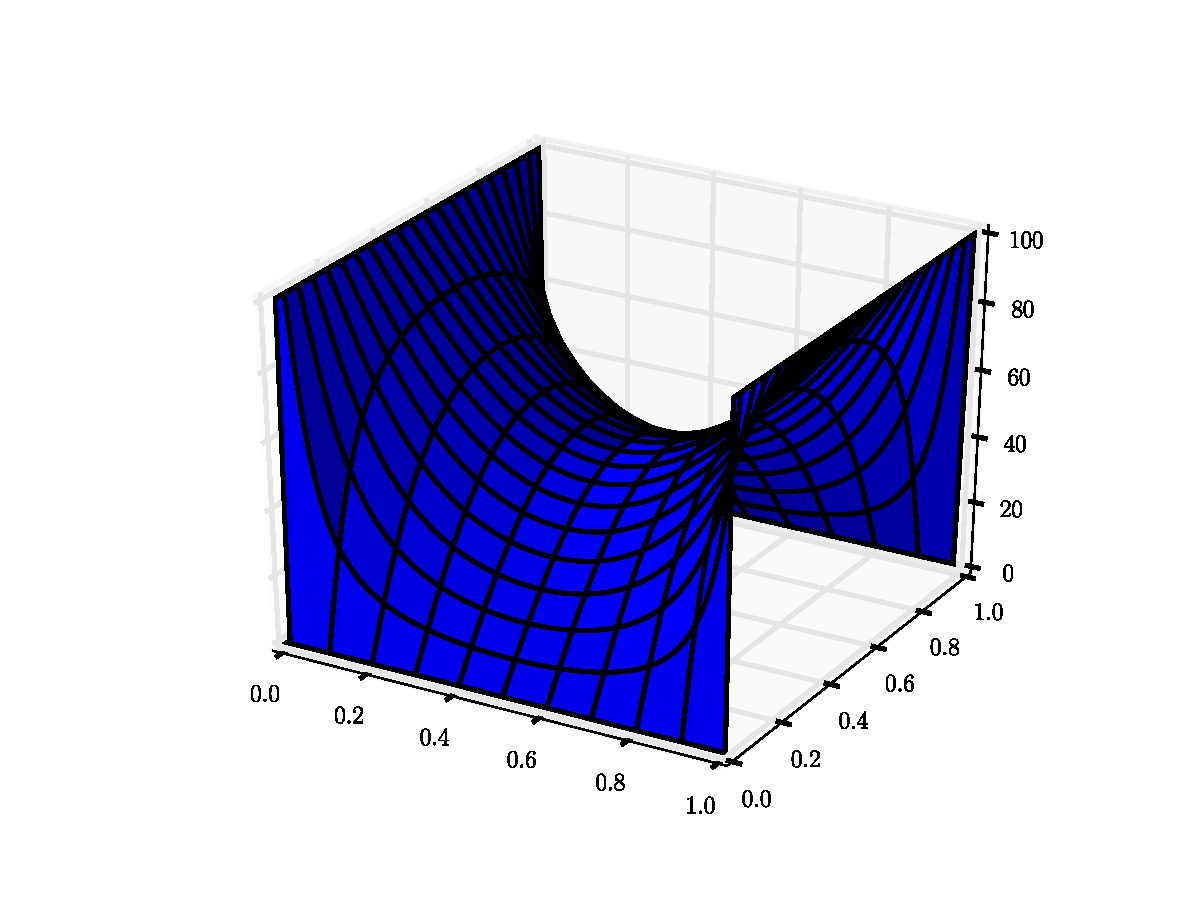
\includegraphics[width=.75\textwidth]{laplace.pdf}
\end{figure}
\end{problem}

\begin{comment}
\section*{Logical Operations}
Logical operations return arrays of only true or false values.
These arrays are often useful in masking values in other arrays.
\begin{lstlisting}
>>> a = np.random.rand(5,5)
>>> a<.5
array([[ True, False, False,  True, False],
       [ True,  True, False,  True, False],
       [False,  True,  True, False, False],
       [False, False,  True, False,  True],
       [ True, False, False,  True, False]], dtype=bool)
>>> a[a<.5]
array([ 0.46121936,  0.11294639,  0.37868745,  0.23435659,  0.25898226,
        0.09095808,  0.19124312,  0.41124911,  0.09823221,  0.03739077,
        0.08655778])
>>> a[a<.3] = 0
>>> a
array([[ 0.46121936,  0.83080909,  0.5632045 ,  0.        ,  0.59581868],
       [ 0.37868745,  0.        ,  0.54977124,  0.        ,  0.753893  ],
       [ 0.79744663,  0.        ,  0.        ,  0.57981239,  0.95839037],
       [ 0.66512744,  0.63471169,  0.41124911,  0.6466058 ,  0.        ],
       [ 0.        ,  0.50692736,  0.54082953,  0.        ,  0.5173614 ]])
\end{lstlisting}
The comparison operators can all be used like this with arrays.
We can quickly test if all elements of a given axis evaluate to true with \li{np.all}.  Likewise, we can test if any element evaluates to true with \li{np.any}.
Because of the nature of floating point numbers, it is next to impossible to accurately test the equality of elements of two arrays.
NumPy provides a special function, \li{np.allclose}, to check if two arrays are \emph{almost} the same (or within some specified tolerances).
\emph{Please note that in some rare cases} \li{np.allclose(a, b)} \emph{will not match} \li{np.allclose(b, a)}.
This is because the equation the function uses for checking closeness is not symmetric ($\abs{a-b} \leq \mbox{atol} + \mbox{rtol}*\abs{b}$).
\begin{lstlisting}
>>> a = np.ones((5, 5))
>>> np.allclose(a, a+1e-5)
True
>>> np.allclose(a, a+1e-4)
False
\end{lstlisting}
NumPy also allows bitwise operations on arrays using the standard Python bitwise operators: \li{&}, \li{|}, and \li{^}, as well as \li{&=}, \li{|=}, and \li{^=}.

\end{comment}

You must keep in mind that the features, operations, and functions discussed in these labs are \emph{most certainly not} an exhaustive list of the things that are included as part of NumPy.
Whenever you need more information you can visit the documentation at \url{http://docs.scipy.org/doc/}

\section*{Methods of NumPy Arrays}
As we have just mentioned, there are \emph{many} different functions included in NumPy that allow you to manipulate arrays.
Some of the most useful ones are also included as methods of array objects  themselves.
If you have not seen methods of objects before, methods are functions that are attached to particular object.
Table \ref{ndarraymethods} shows some of the more common methods of NumPy arrays.
A more comprehensive list can be found at \url{http://docs.scipy.org/doc/numpy/reference/generated/numpy.ndarray.html}

\begin{table}[h]
\centering
	\begin{tabular}{l|p{10cm}}

    \hline

    Function & Description \\

    \hline

    \li{all} & returns True if all elements evaluate to True \\

    \li{any} & returns True if any elements evaluate to True \\

    \li{argmax} & indices of maximum value(s) \\

    \li{argmin} & indices of minimum value(s) \\

    \li{argsort} & indices that would sort the array \\

    \li{astype} & casts a copy of an array to a different data type \\

    \li{clip} & restrict values in an array to fit within a given range \\

    \li{conj} & return the complex conjugate of the array \\

    \li{copy} & return a copy of the array\\

    \li{diagonal} & return a given diagonal of the array \\

    \li{dot} & matrix multiplication \\

    \li{max} & max element of the array \\

    \li{mean} & average of the array \\

    \li{min} & minimum element of the array \\

    \li{prod} & product of elements of the array \\

    \li{ravel} & make a flattened version of an array, return a view if possible \\

    \li{reshape} & return a view of the array with a changed shape \\

    \li{round} & return a rounded version of the array \\

    \li{sort} & sort the array in place \\

    \li{std} & compute the standard deviation \\

    \li{sum} & sum the elements of the array \\

    \li{swapaxes} & return a view with the given axes swapped \\

    \li{tolist} & return the array represented as a list or nested list \\

    \li{trace} & return the sum of the elements along the main diagonal \\

    \li{var} & return the variance of the array \\

    \hline

    \end{tabular}
\caption{A few of the methods of NumPy arrays.}
\label{ndarraymethods}
\end{table}

Many of these methods allow you to specify an axis along which to operate, for example: \li{A.mean(axis=0)} computes the average of each row of \li{A}.
Here are a few examples of how to use these methods.
\begin{lstlisting}
>>> import numpy as np
>>> from numpy.random import rand, randint
>>> A = randint(0, 10, (4,4)) # a 4x4 array of random integers in [0, 10)
>>> A
array([[6, 6, 2, 2],
       [1, 1, 0, 8],
       [8, 3, 6, 8],
       [1, 4, 9, 0]])
>>> A.max(axis=0) # maximum row, i.e. the maximum element of each column
array([8, 6, 9, 8])
>>> A.dot(A) # matrix multiplication of A with itself
array([[ 60,  56,  42,  76],
       [ 15,  39,  74,  10],
       [107, 101, 124,  88],
       [ 82,  37,  56, 106]])
>>> A.sum(axis=1) # sum of columns, i.e. sum along each row
array([16, 10, 25, 14])
\end{lstlisting}

\begin{problem}
% There should be more problems like this in the vectorization lab.
% I'll include this one here for now though.
Write a function which, given an integer $n$, makes an $n\times n$ array of random normally distributed floating point values, computes the mean along each row, then computes the variance of these means.
The computation of the variance should only take one line. The function should return the variance.
As you increase the value of n what do you notice about the output of the function?
This illustrates one version of the Law of Large Numbers, about which you will learn more later on.
\end{problem}

\section*{Saving Arrays}
It is often useful to save an array as a file.
NumPy provides several easy methods for saving and loading array data.
\begin{table*}[h]
\begin{tabular}{l|l}
\hline
\li{np.save(file, arr)} & Save an array to a binary file \\
\li{np.savez(file, *arrs)} & Save multiple arrays to a binary file \\
\li{np.savetxt(file, arr)} & Save an array to a text file \\
\hline
\end{tabular}
\end{table*}

\begin{table*}[h]
\begin{tabular}{l|l}
\hline
\li{np.load(file)} & Load and return an array from a binary file \\
\li{np.loadtxt(file)} & Load and return an array from text file \\
\hline
\end{tabular}
\end{table*}

Let's practice saving an array to a file and loading it again.
Note that, when saving an array, NumPy automatically appends the extension \li{.npy} if it is not already present.
\begin{lstlisting}
a = np.arange(30)
np.save('test_arr', a)
new_a = np.load('test_arr.npy')
np.savez('test_multi', a=a, new_a=new_a)
arrs = np.load('test_multi.npz')
\end{lstlisting}
The variable \li{arrs} points to a dictionary object with the keys \li{a} and \li{new_a} which reference the arrays that have been saved.
The \li{.npz} file extension is the file type used to store multiple arrays.